\documentclass{article}
\usepackage{graphicx} % Required for inserting images
\usepackage{titling} % For \subtitle command
\graphicspath{{images/}} %configuring the graphicx package
\usepackage{hyperref}

\title{Laboratório de Engenharia de Software}




\date{Setembro 2025}

\author{Bruno Antico Galin - 10417318 \and 
Davi Martins Figueiredo - 10374878 \and
Gustavo Fugulin Soares da Silva - 10418552 \and
Henrique Pena Ribeiro - 10417975 \and
Joao Pedro Gianfaldoni - 10409524}



\begin{document}

\maketitle
\newpage


\tableofcontents

\newpage



\section{Introdução}
IADvogado é uma iniciativa tecnológica que busca democratizar o acesso à Justiça no Brasil por meio de Inteligência Artificial. A proposta consiste em um sistema capaz de traduzir documentos jurídicos — petições, decisões e andamentos processuais — em linguagem clara e acessível para a população.

A solução é acessível via WhatsApp e, futuramente, por meio de aplicativo dedicado, oferecendo respostas em formato texto e áudio para aumentar a inclusão de pessoas com baixa escolaridade, idosos e cidadãos com deficiência visual.

O projeto tem como foco principal reduzir as barreiras de entendimento que afastam os cidadãos de seus direitos, promovendo transparência e cidadania. Além disso, a iniciativa está alinhada aos seguintes Objetivos de Desenvolvimento Sustentável (ODS) da ONU:
\begin{itemize}
    \item ODS 10 – Redução das Desigualdades: ao oferecer acessibilidade jurídica para populações vulneráveis.
    \item ODS 16 – Paz, Justiça e Instituições Eficazes: ao promover maior transparência, acesso à informação e fortalecimento da confiança no sistema judicial.
    \item ODS 9 – Indústria, Inovação e Infraestrutura: ao utilizar tecnologia para ampliar o impacto social e construir soluções inclusivas e escaláveis
\end{itemize}

\section{Definição da demanda}
    \subsection{Oportunidade Percebida}
    O problema identificado está na dificuldade de compreensão dos documentos jurídicos por parte da população em geral. Petições, decisões e andamentos processuais utilizam uma linguagem técnica, repleta de jargões e formalismos, o que torna o entendimento inacessível para pessoas sem formação jurídica. Esse obstáculo afeta principalmente cidadãos com baixa escolaridade, idosos e pessoas com deficiência visual, que acabam encontrando barreiras para exercer plenamente seus direitos. A falta de clareza nos textos jurídicos compromete a autonomia e a transparência no acompanhamento de processos legais.
    \subsection{Razão ou justificativa para esta demanda}
    A justificativa para o desenvolvimento da solução está na necessidade de democratizar o acesso à justiça, tornando a linguagem jurídica mais clara e compreensível para todos. Ao simplificar os documentos legais, busca-se reduzir desigualdades, garantir que o cidadão compreenda prazos, obrigações e consequências de cada etapa do processo, além de ampliar a acessibilidade por meio de recursos como a conversão de texto em áudio. Esse objetivo também dialoga com a promoção da cidadania, beneficiando indivíduos e instituições como a Defensoria Pública e organizações que atendem populações vulneráveis, além de estar alinhado a metas sociais e aos Objetivos de Desenvolvimento Sustentável da ONU.

\subsection{Descrição sucinta do produto de software que será produzido }
O software a ser desenvolvido, denominado \textbf{IADvogado}, terá como finalidade traduzir documentos jurídicos em uma linguagem simples, acessível e direta para o público leigo. Inicialmente, o sistema será disponibilizado por meio de integração com o WhatsApp, possibilitando que o usuário envie documentos ou insira o número de um processo para receber a explicação. O funcionamento será apoiado em tecnologias como OCR para leitura de documentos, modelos de linguagem para simplificação textual e TTS para oferecer versões em áudio. O produto, em sua versão mínima viável (MVP), fornecerá explicações organizadas em três blocos principais — o que aconteceu, o que significa e o que fazer agora — acompanhadas de mensagens de responsabilidade que deixam claro que a ferramenta não substitui um advogado. 

\subsection{Clientes, usuários e demais envolvidos }
\begin{tabular}{|p{6cm}|p{6cm}|}
    \hline
    \centering \textbf{Grupo} & \textbf{Características / Relação com o produto}\\ \hline
    Cidadãos em processos simples (trabalhistas, previdenciárias, pequenas causas) & Usuários finais: aqueles que necessitam entender seus processos, decisões, petições. \\\hline
    Pessoas com baixa escolaridade, idosos, deficiência visual &Também usuários finais, com requisitos especiais de acessibilidade (áudio, clareza, simplicidade).\\\hline
    Defensoria Pública e ONGs &Instituições que podem usar a ferramenta para facilitar comunicação com assistidos, reforçar transparência, reduzir carga de explicação/manual. \\\hline
    Advogados / operadores do direito &Impactados indiretamente: embora o sistema não substitua advogados, eles poderão ter cidadãos mais bem informados, talvez menos dúvidas repetitivas, etc. \\\hline
    Time de desenvolvimento / mantenedores &Responsáveis pela implementação técnica, design, qualidade, manutenção, ética e conformidade legal (como LGPD). \\\hline
    Órgãos regulatórios / ética jurídica &Podem ter interesse na conformidade, na limitação de escopo (não substituir advogado), proteção de dados. \\\hline
\end{tabular}

\subsection{ Principais etapas necessárias para construir este produto}

As principais etapas para o desenvolvimento do sistema são:

\begin{itemize}
    \item \textbf{Levantamento de requisitos:} Identificação das funcionalidades principais, como tradução de documentos jurídicos, uso de OCR, geração de áudio e integração com o WhatsApp.
    \item \textbf{Definição do escopo e MVP:} Seleção das funcionalidades prioritárias que entreguem valor imediato ao usuário.
    \item \textbf{Modelagem:} Estruturação da arquitetura do sistema, fluxos de interação e organização dos dados.
    \item \textbf{Implementação:} Desenvolvimento da infraestrutura backend, integração com serviços externos e interface de comunicação com os usuários.
    \item \textbf{Testes:} Verificação funcional, usabilidade, desempenho, acessibilidade e conformidade com a legislação.
    \item \textbf{Lançamento do MVP:} Disponibilização inicial para um grupo piloto, coleta de feedback e melhorias.
    \item \textbf{Manutenção e evolução:} Atualizações contínuas, correções de falhas e expansão de funcionalidades.
\end{itemize}

\subsection{Principais critérios de qualidade para o produto}

Os principais critérios de qualidade definidos para o produto são:

\begin{itemize}
    \item \textbf{Clareza e compreensibilidade:} Linguagem simples e acessível, livre de jargões jurídicos.
    \item \textbf{Acessibilidade:} Inclusão de recursos como áudio e interfaces intuitivas.
    \item \textbf{Confiabilidade:} Explicações corretas, sem ambiguidades que possam causar interpretações equivocadas.
    \item \textbf{Tempo de resposta:} Rapidez no processamento e na entrega das informações.
    \item \textbf{Segurança e privacidade:} Conformidade com a LGPD e proteção rigorosa dos dados fornecidos pelos usuários.
    \item \textbf{Robustez:} Capacidade de lidar com diferentes formatos de documentos e possíveis falhas de OCR.
    \item \textbf{Usabilidade:} Interface simples e intuitiva, adequada a diversos perfis de usuários.
    \item \textbf{Escalabilidade:} Suporte ao crescimento da base de usuários e ampliação das funcionalidades.
    \item \textbf{Ética e legalidade:} Garantia de que o sistema não substitua advogados, servindo apenas como apoio informativo.
\end{itemize}

\section{Requisitos do produto}
\subsection*{Requisitos Funcionais}
\begin{tabular}{|c|p{7cm}|c|c|}
\hline
\textbf{ID} & \textbf{Descrição} & \textbf{Prioridade} & \textbf{Categoria} \\
\hline
RF01 & Receber documentos (PDF, imagem, texto) e gerar explicação simplificada. & Alta & Funcionalidade principal \\\hline
RF02 & Estruturar explicações em três blocos: O que aconteceu, O que significa, O que fazer agora. & Alta & Experiência do usuário \\\hline
RF03 & Permitir consulta por número de processo. & Alta & Entrada de dados \\\hline
RF04 & Retornar conteúdo em formato textual no canal de interação. & Alta & Saída \\\hline
RF05 & Gerar resposta opcional em formato de áudio (TTS). & Alta & Acessibilidade \\\hline
RF06 & Notificar automaticamente o usuário sobre novos andamentos. & Média & Usabilidade \\\hline
RF07 & Suporte inicial no WhatsApp, expansível para PWA/mobile. & Média & Multicanalidade \\\hline
RF08 & Registrar logs de uso, erros e tempo de resposta. & Alta & Monitoramento \\\hline
RF09 & Incluir disclaimers legais em todas as respostas. & Alta & Ética/Compliance \\\hline
RF10 & Oferecer autenticação mínima (telefone ou conta) para acompanhamento contínuo. & Média & Segurança \\\hline
RF11 & Permitir configuração de preferências (texto, áudio ou ambos). & Média & Personalização \\\hline
RF12 & Disponibilizar histórico de consultas armazenado por período definido. & Média & Usabilidade \\\hline
RF13 & Suporte a múltiplos idiomas. & Baixa & Internacionalização \\\hline
RF14 & Garantir compatibilidade com diferentes dispositivos e navegadores. & Alta & Compatibilidade \\\hline
RF15 & Implementar sistema de feedback para melhorias contínuas. & Baixa & Qualidade \\
\hline
\end{tabular}

\subsection*{Requisitos não funcionais}
\begin{tabular}{|c|p{7cm}|c|c|}
\hline
\textbf{ID} & \textbf{Descrição} & \textbf{Prioridade} & \textbf{Categoria} \\
\hline
RNF01&	Respostas devem ser compreensíveis a cidadãos com escolaridade média ou inferior.&	Alta&	Usabilidade\\\hline
RNF02& Tempo máximo de resposta: 2 minutos&.	Alta&	Desempenho\\\hline
RNF03&	Oferecer suporte a áudio e design responsivo para acessibilidade.&	Alta&	Acessibilidade\\\hline
RNF04&	Acuracia mínima das traduções simplificadas 90	&Alta &	Confiabilidade\\\hline
RNF05&	Suportar múltiplos usuários simultâneos sem degradação perceptível.&	Alta&	Escalabilidade\\\hline
RNF06&	Criptografia em repouso e em trânsito; exclusão periódica de dados.	&Alta&	Segurança\\\hline
RNF07&	Implantável em diferentes nuvens (Railway, Digital Ocean, AWS).	&Média	&Portabilidade\\\hline
RNF08&	Compatibilidade com navegadores modernos e Android/iOS.	&Média	&Compatibilidade\\\hline
RNF09&	Código modular, documentado e testado (PEP8, docstrings, testes unitários).&	Alta	&Manutenibilidade\\\hline
RNF10&	Disponibilidade mínima de 99 ao mês.	&Alta	&Confiabilidade\\\hline
RNF11&	Registro de acessos e operações para auditoria.	&Média	&Auditabilidade\\\hline
RNF12&	Suporte futuro para múltiplos idiomas (internacionalização).&	Baixa&	Evolução\\\hline
RNF13&	Uso preferencial de serviços open source e infraestrutura de baixo custo.&	Média&	Sustentabilidade financeira\\\hline
RNF14&	Reforço constante de disclaimers para conformidade legal (OAB, LGPD).&	Alta&	Ética/Compliance\\\hline
\end{tabular}
\subsection*{Restrições}
\begin{tabular}{|c|p{7cm}|c|c|}
\hline
\textbf{ID} & \textbf{Descrição} & \textbf{Prioridade} & \textbf{Categoria} \\
\hline
RE01&	O sistema não pode elaborar petições ou peças jurídicas.&	Alta&	Legal\\\hline
RE02&	O sistema não pode emitir parecer jurídico personalizado.&	Alta&	Legal\\\hline
RE03&	Dados devem seguir integralmente a LGPD.&	Alta	&Conformidade\\\hline
RE04&	A infraestrutura inicial deve operar em modelo de baixo custo.&	Média&	Operacional\\
\hline
\end{tabular}

\newpage

\section{Wireframes}

\subsection*{Tela Principal (Versão Desktop/Web e Mobile)}
Protótipo da tela inicial onde o usuário interage com o sistema IADvogado. No desktop, os elementos aparecem organizados em uma interface ampla, enquanto no mobile o layout é simplificado e adaptado para telas menores, com botões mais acessíveis ao toque. Essa tela inclui opções como envio de documentos, consulta de processo e visualização de respostas. 

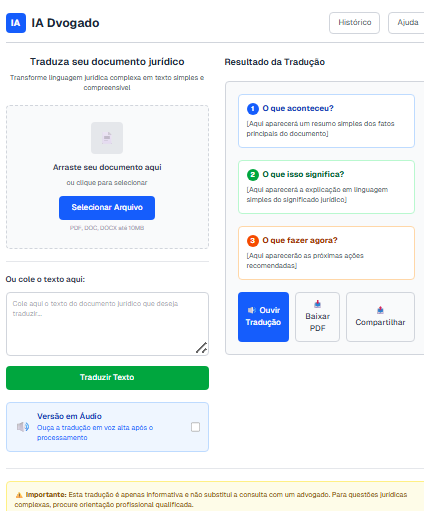
\includegraphics{images/488857524-513c5783-90a3-4785-a3a8-041214390468.png}

\newpage

\subsection*{Interface do sistema IADvogado com WhatsApp}
Mostra como a interação via WhatsApp será modelada: simula mensagens em que o usuário envia um documento ou número de processo e recebe de volta uma explicação simplificada, possivelmente com opção em áudio ou texto.
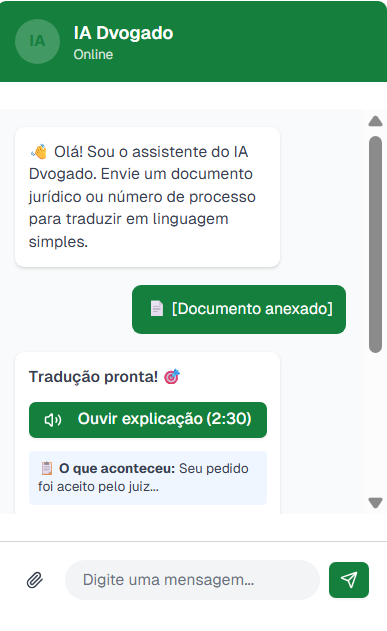
\includegraphics{images/488854020-5cb044cf-bd2e-463b-be56-70f556ed3ffc.png}
\newpage

\subsection*{Tela Inicial em um app futuro}
Protótipo de uma tela inicial caso o sistema evolua para um aplicativo dedicado. Exibe o logo e opções principais, como “Enviar documento”, “Consultar processo” e “Histórico”.

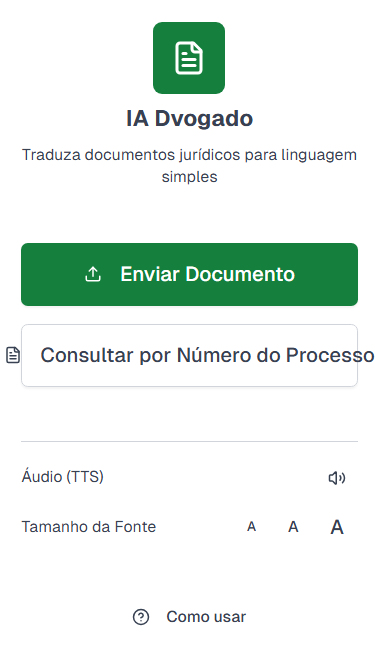
\includegraphics{images/488854265-1f3c3198-5f5b-492a-85b2-fcf826105ffa.png}

\subsection*{Tela de Resultado (tradução simplificada)}
Mostra como será exibida a saída: após o envio de documento ou consulta, o sistema retorna uma tradução simplificada em blocos — o que aconteceu, o que significa e o que fazer agora.

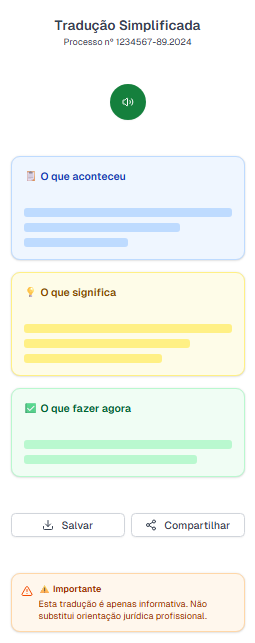
\includegraphics{images/488854473-c9885c0e-2982-4055-8b41-44baeb4fe4d0.png}


\section{Modelagem}
\subsection{Propósito da Modelagem}
Esta seção oferece um esboço integrador do sistema, antecipando seu aspecto arquitetural, como os componentes se encaixam e como os requisitos se materializam em casos de uso, dados, interfaces e processos. O objetivo é reduzir ambiguidades, orientar decisões de design e facilitar a comunicação entre stakeholders técnicos e não técnicos.

\subsection{Escopo e Fronteira do Sistema}
\begin{itemize}
    \item \textbf{Nome do Sistema:} Justiça Simples
    \item \textbf{Fronteira:} Serviço de tradução/simplificação jurídica acessível inicialmente via Whatsapp (Evolution API) e futuramente PWA/Mobile.
    \item \textbf{Atores Externos:} Usuário final (cidadão), Defensoria/ONG parceira (operador institucional), Provedores de OCR/TTS/LLM, Portais/Jurisdições (TJs/TRTs/INSS), Plataforma WhatsApp (Evolution API), Serviço de armazenamento seguro (BD/objeto).
    \item \textbf{Visão de alto nível do fluxo:} Usuário envia documento/número de processo → sistema extrai texto (OCR) → simplifica (LLM) → estrutura saída → gera áudio (TTS) → devolve texto/áudio → registra logs/métricas.
\end{itemize}
\subsection{Diagrama de Contexto}
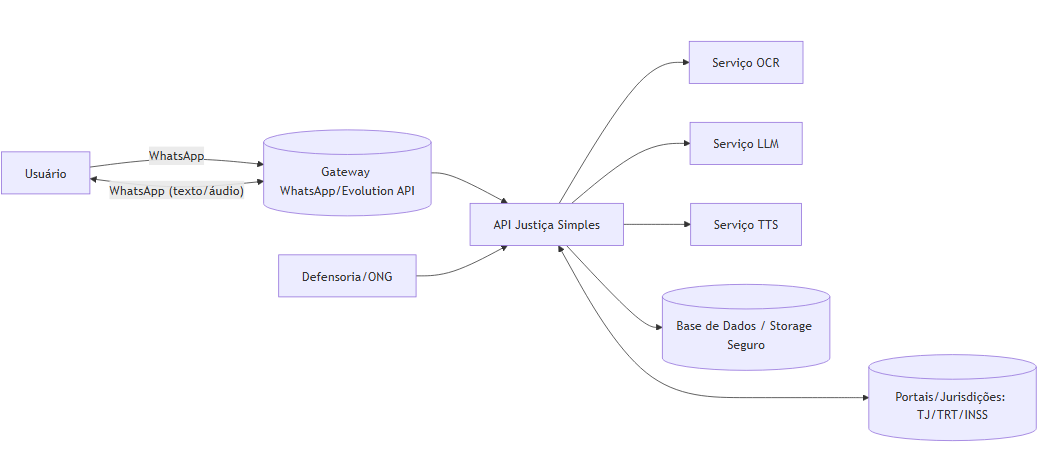
\includegraphics[width=2\textwidth,height=6cm,keepaspectratio]{images/486130606-99068cfc-9977-4b36-b273-cd742f36880f.png}
\newpage
\subsection{Modelo de Caso de Uso}

\subsubsection{Diagrama de Casos de Uso (visão resumida)}
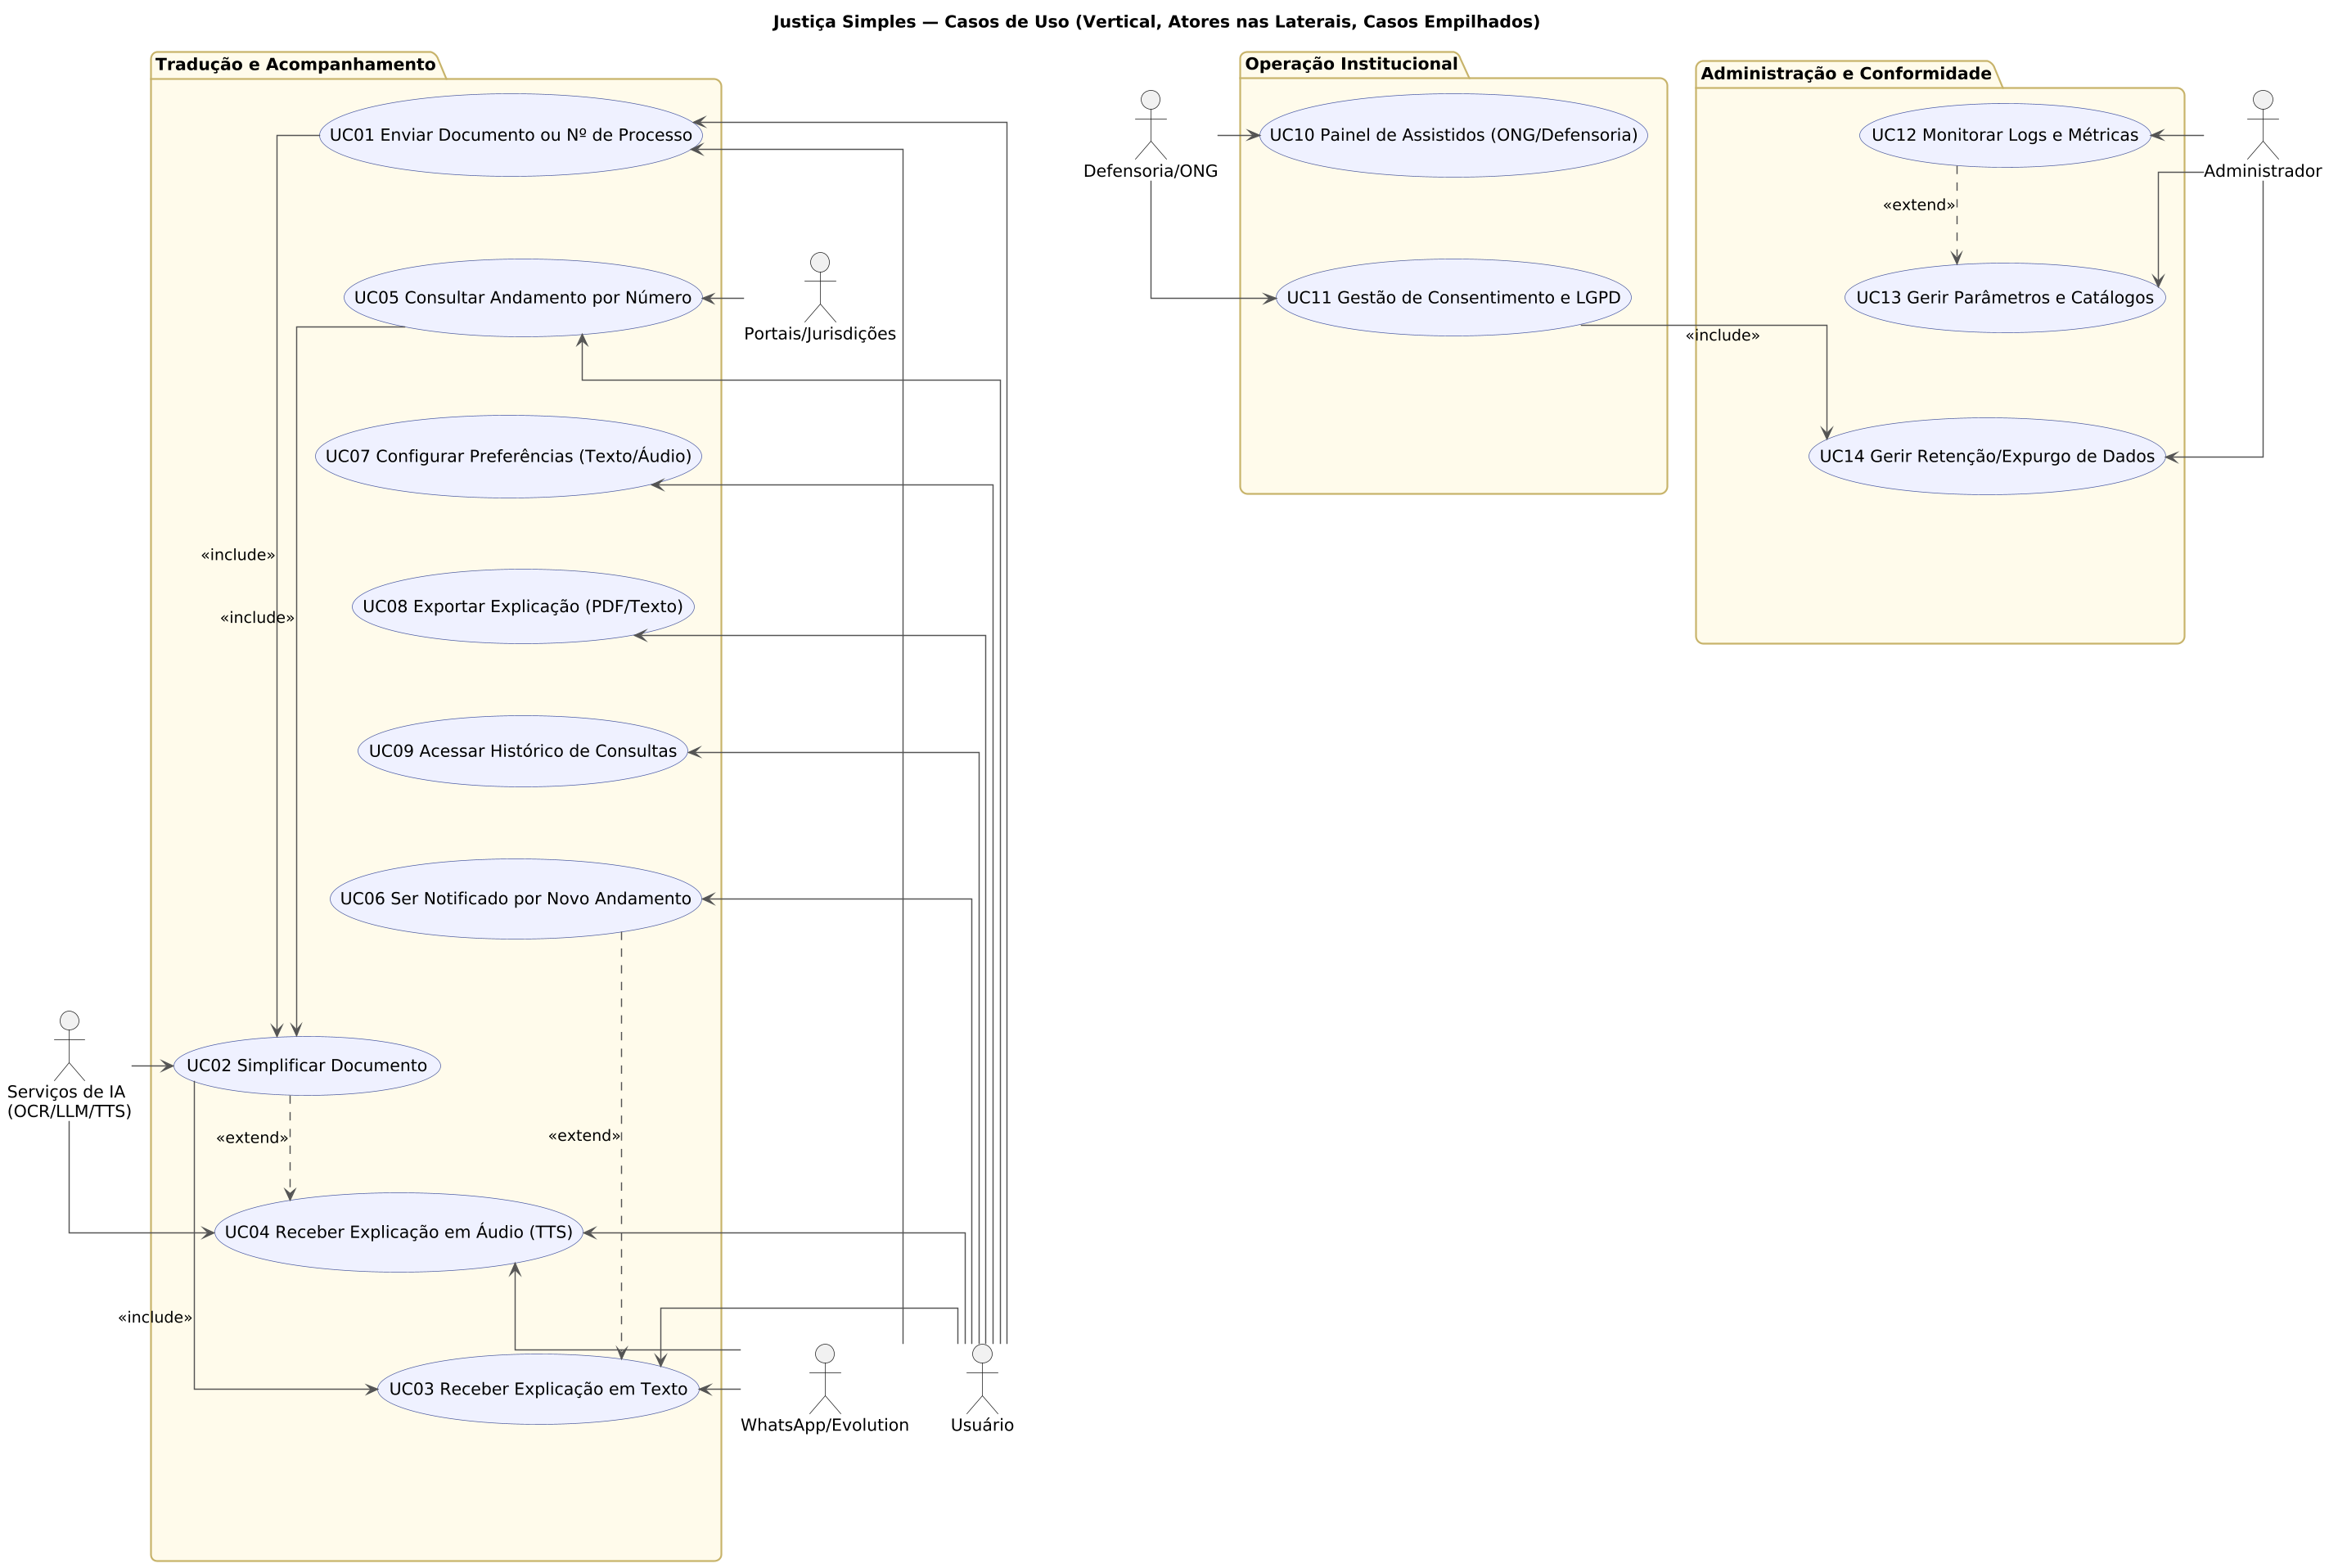
\includegraphics[width=1.25\textwidth,height=10cm,keepaspectratio]{images/488857090-49e54eee-2d6e-499b-9600-ad69237805b8.png}
\subsubsection{Caso de Uso Crítico (Completo)}
\begin{itemize}
    \item \textbf{Atores Principais: }Usuário (A1).
    \item \textbf{Pré-Condições: }Usuário autenticado (mínimo: validação de telefone) e consentimento LGPD.
    \item \textbf{Cenário de sucesso Principal:}
    \begin{enumerate}
        \item Usuário envia PDF/Imagem/Texto via Whatsapp.
        \item Sistema recebe e valida formato; registra pedido.
        \item Sistema executa OCR (se aplicável) e extrai texto.
        \item Sistema aplica prompt/heurística e submete a LLM.
        \item Sistema estrutura resposta em blocos: “O que aconteceu / O que significa / O que fazer agora”.
        \item Sistema devolve texto ao usuário.
        \item Opcionalmente, o usuário solicita áudio; sistema gera TTS e envia nota de voz.
    \end{enumerate}

    \item \textbf{Cenário Alternativos}
    \begin{itemize}
        \item 4a. OCR falha → sistema solicita novo envio (qualidade) ou oferece tentativa de leitura manual.
        \item 5a. LLM indisponível → fallback para fila assíncrona e notificação de indisponibilidade.
        \item 7a. TTS indisponível → instruir leitura em voz do dispositivo (fallback).
    \end{itemize}
    \item \textbf{Restrições/Observações:} Inserir disclaimer de que não há consultoria jurídica personalizada.
\end{itemize}

\subsection{Modelo de Sequência (Fluxo Principal do MVP)}
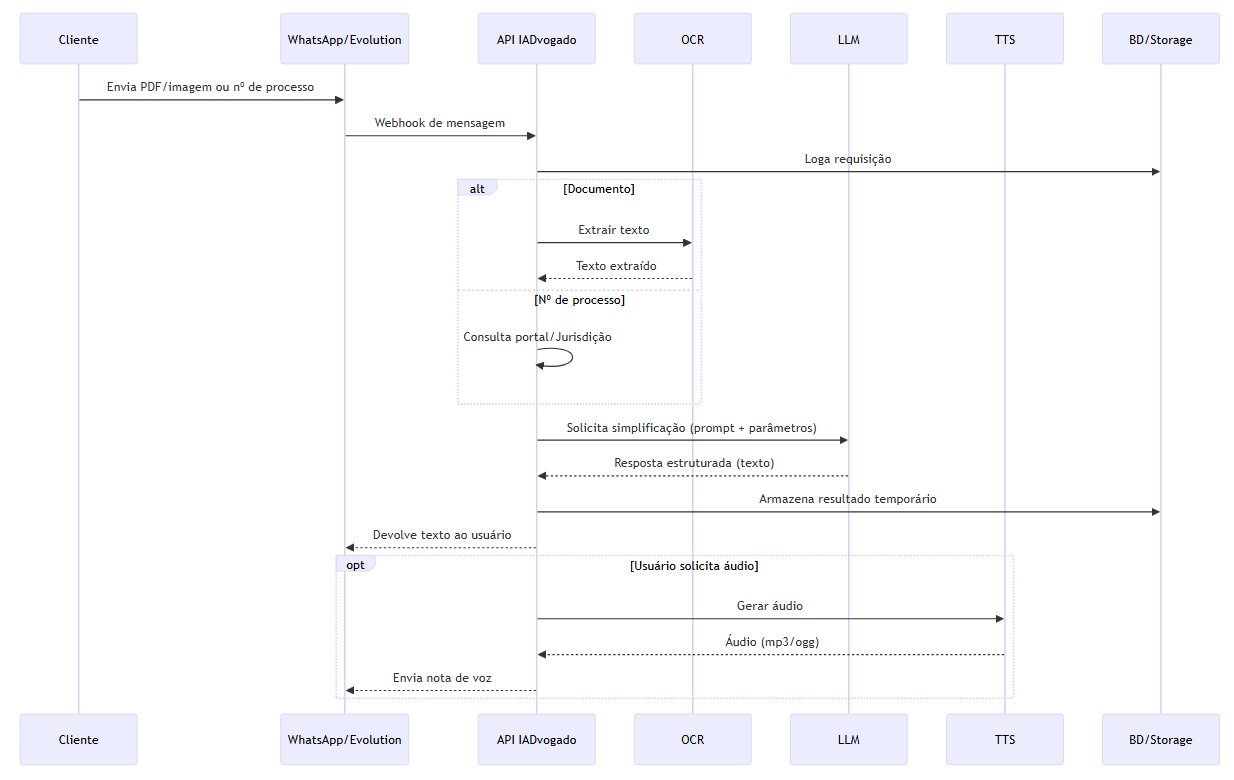
\includegraphics[width=9\textwidth,height=7cm,keepaspectratio]{images/488839370-73a99421-2751-4901-8dad-6b8227931d8f.png}

\subsection{Modelo de Classes}
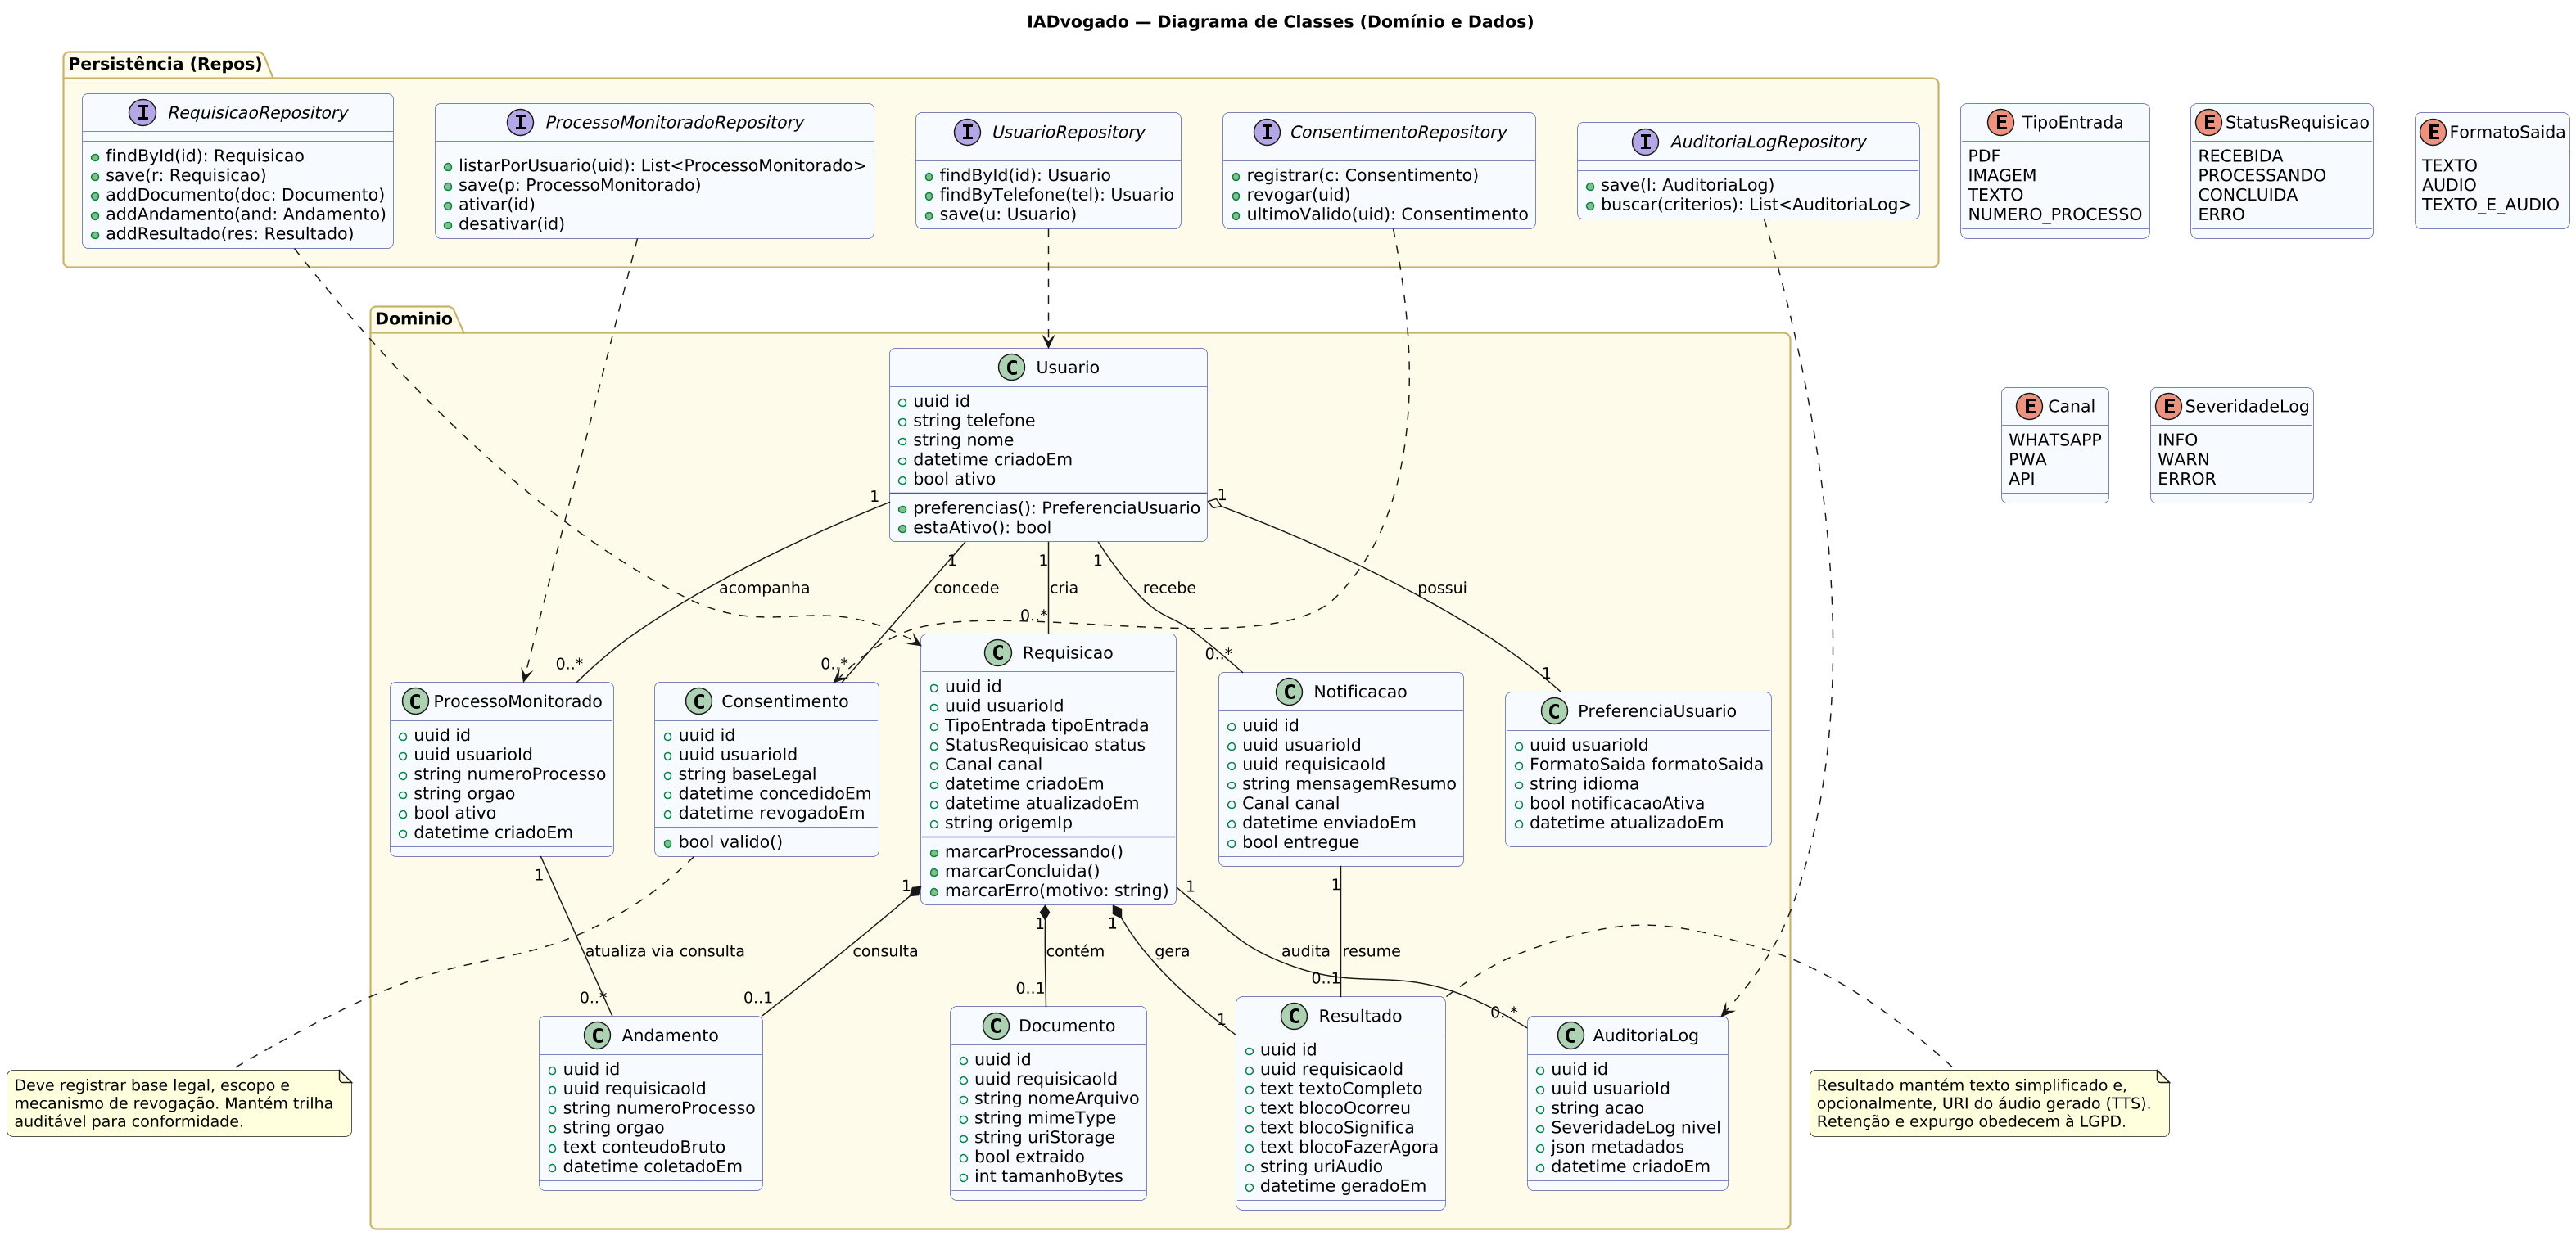
\includegraphics[width=9\textwidth,height=7cm,keepaspectratio]{images/488859339-e96e68b8-5b16-4772-ad8f-b181fcb76a5d.png}
\subsubsection{Modelo de Classes - Integrações do Sistema}
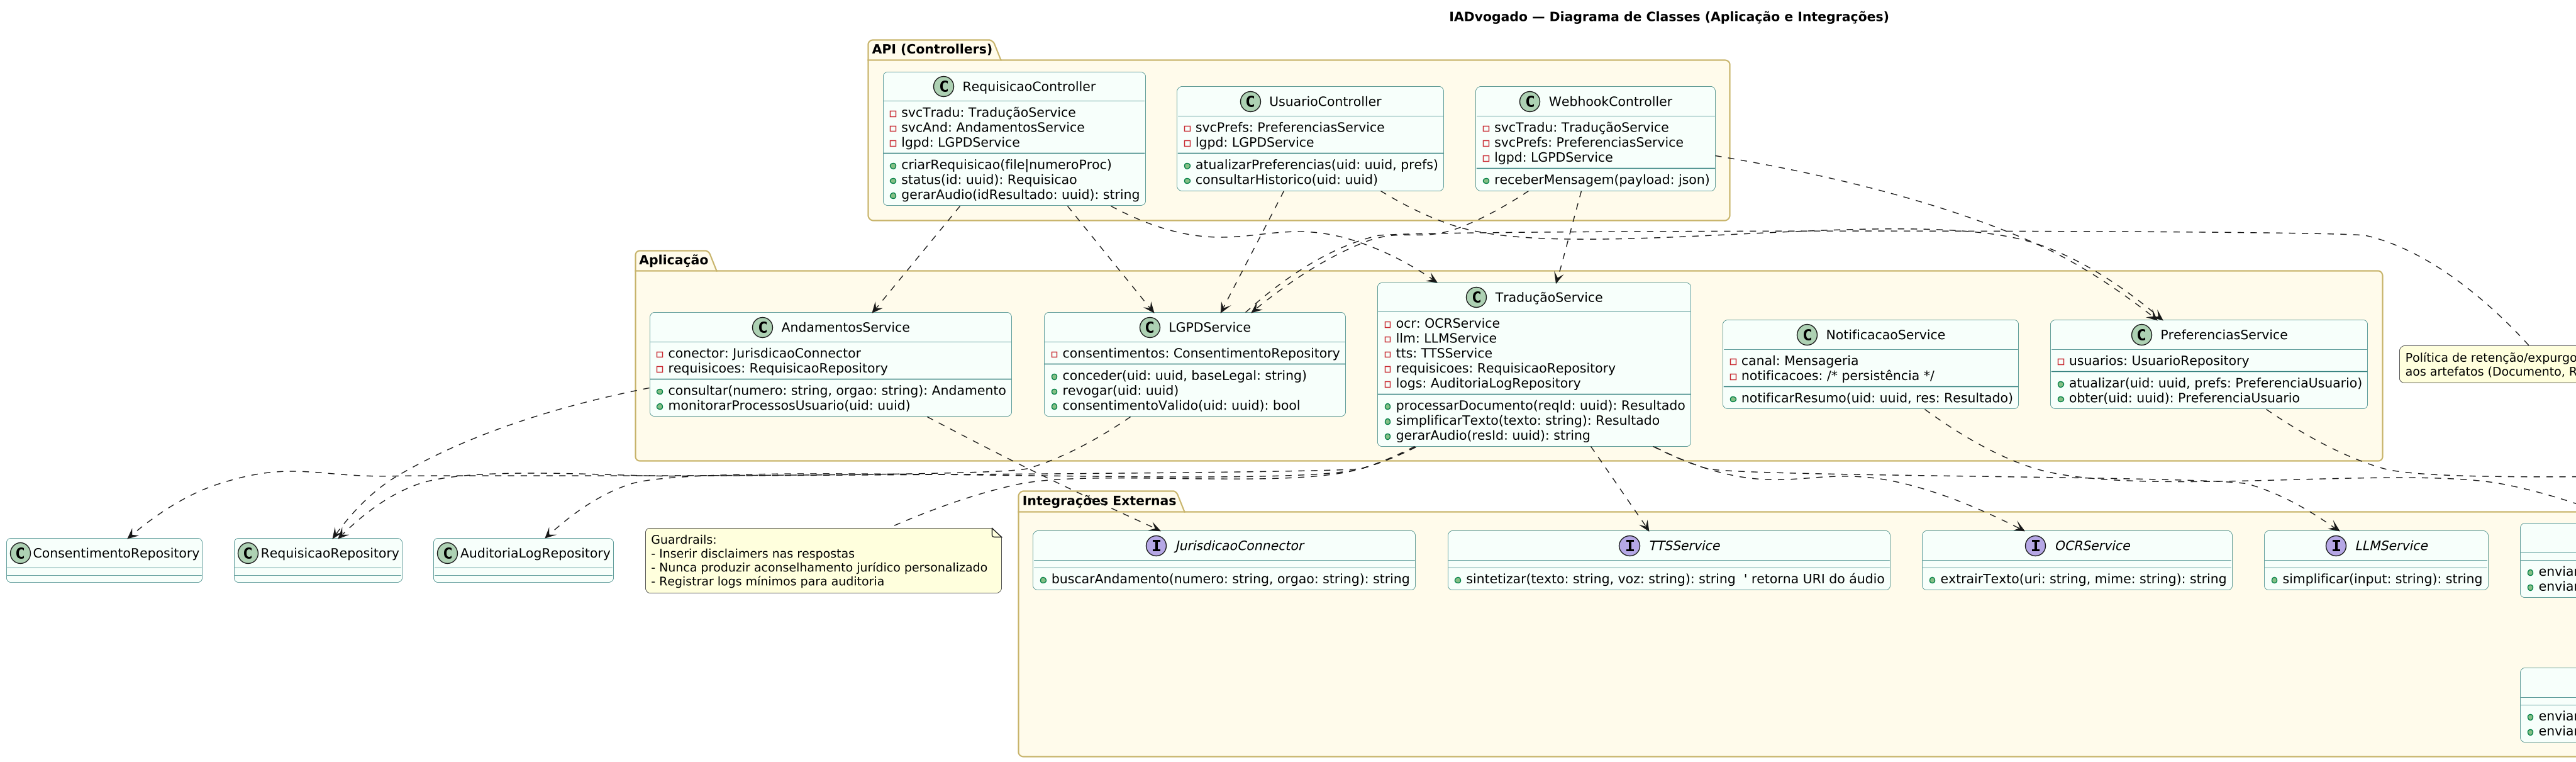
\includegraphics[width=1.3\textwidth,height=7cm,keepaspectratio]{images/488860207-8dae7c6e-94d9-4128-88ce-490bab98ead1.png}

\newpage

\subsection{Modelos de Dados (ER Simplificado)}
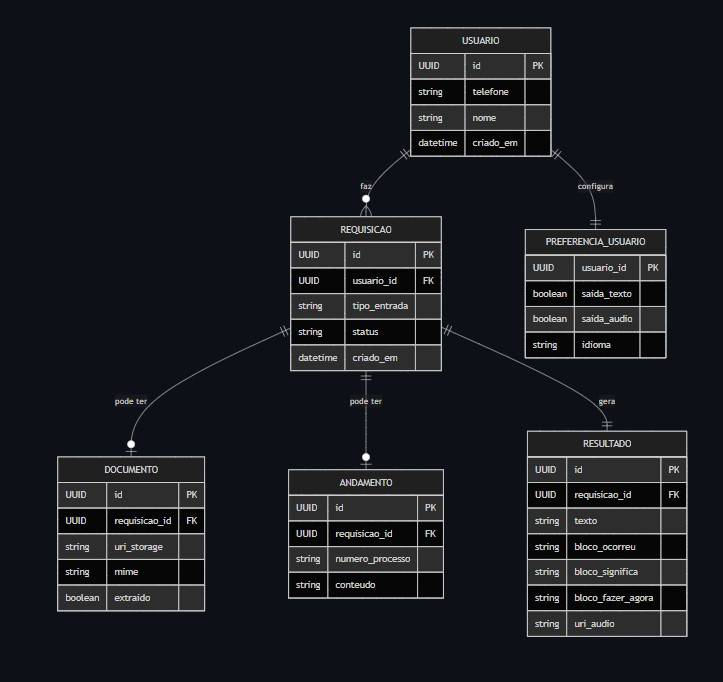
\includegraphics[width=3\textwidth,height=8cm,keepaspectratio]{images/Modelo-de-Dados.jpg}

\textbf{Nota:} chaves/relacionamentos mínimos para MVP; versionamento de esquema via migrações.

\subsection{Modelo de Estados (Requisição)}
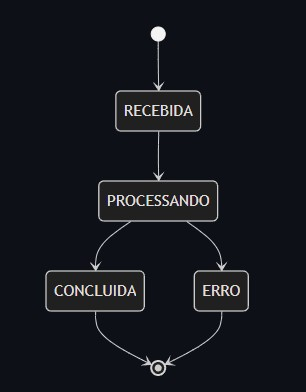
\includegraphics[width=3\textwidth,height=7cm,keepaspectratio]{images/Modelo-de-Estados.jpg}

\textbf{Eventos típicos:} arquivo recebido, OCR ok, LLM ok, TTS ok, falha externa.

\newpage

\section{Arquitetura do Sistema}

A linguagem de programação a ser usada no sistema é Python 3.11, com uma integração de API.

\subsection{Modelo de Componentes (Arquitetura Lógica)}
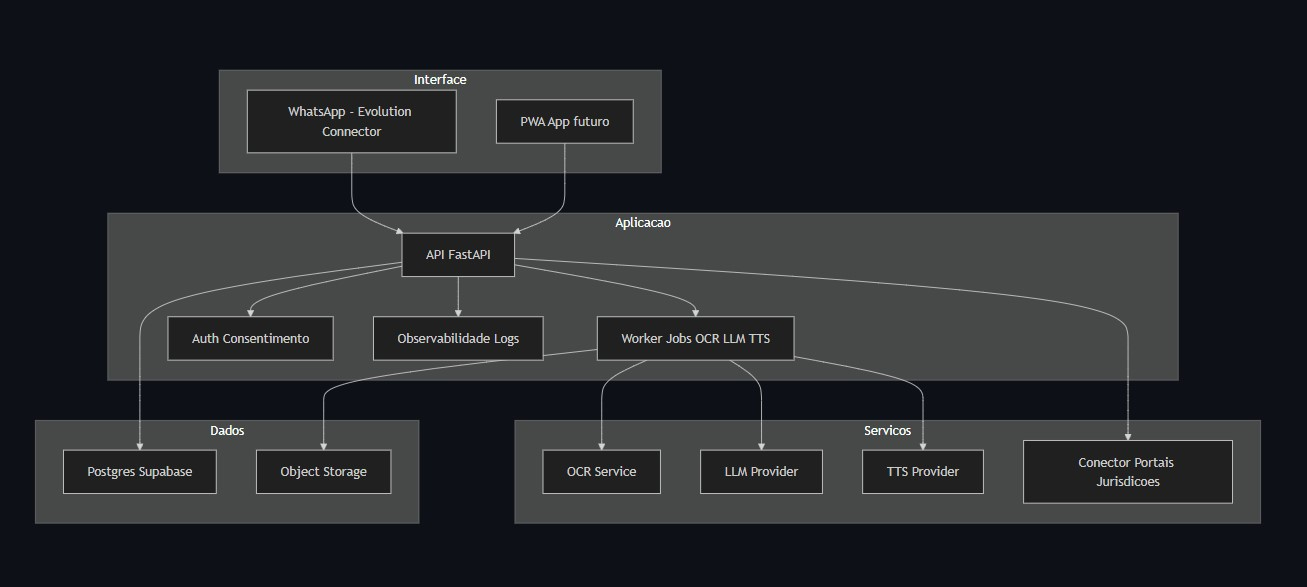
\includegraphics[width=1.3\textwidth,height=7cm,keepaspectratio]{images/Modelo-de-Componentes.jpg}
\textbf{Racional:} separação de interface, aplicação, serviços externos e dados, favorecendo escalabilidade, testabilidade e DevOps.

\subsection{Modelo de Implantação (Deployment - esboço)}
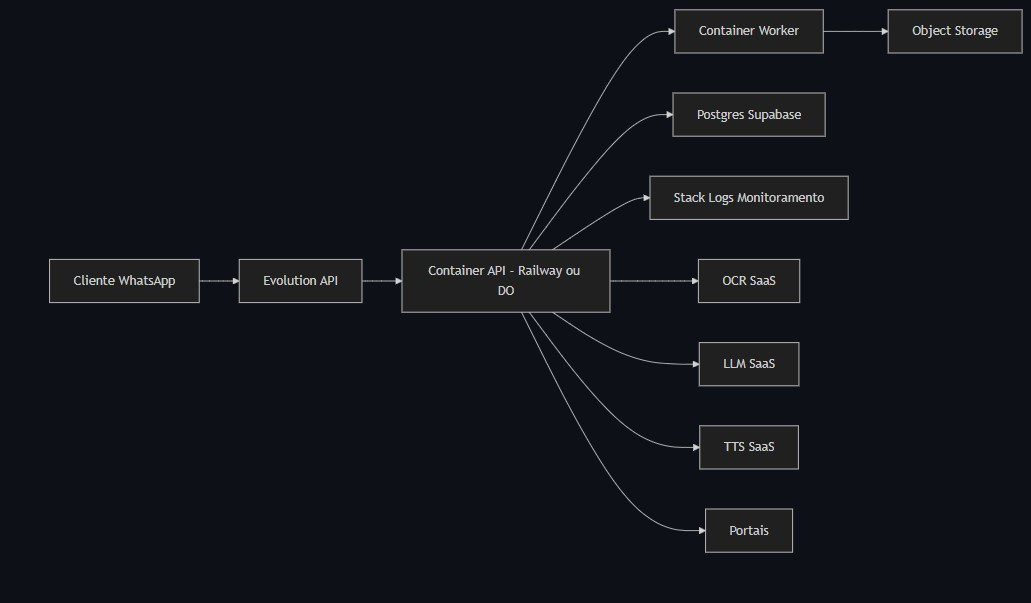
\includegraphics[width=1.4\textwidth,height=7cm,keepaspectratio]{images/Modelo-de-Implantacao.jpg}
\textbf{Observações de DevOps: } integração/entrega contínua, logs/monitoramento, automação de infraestrutura e segurança na pipeline.

\subsection{Modelo de Pacotes}
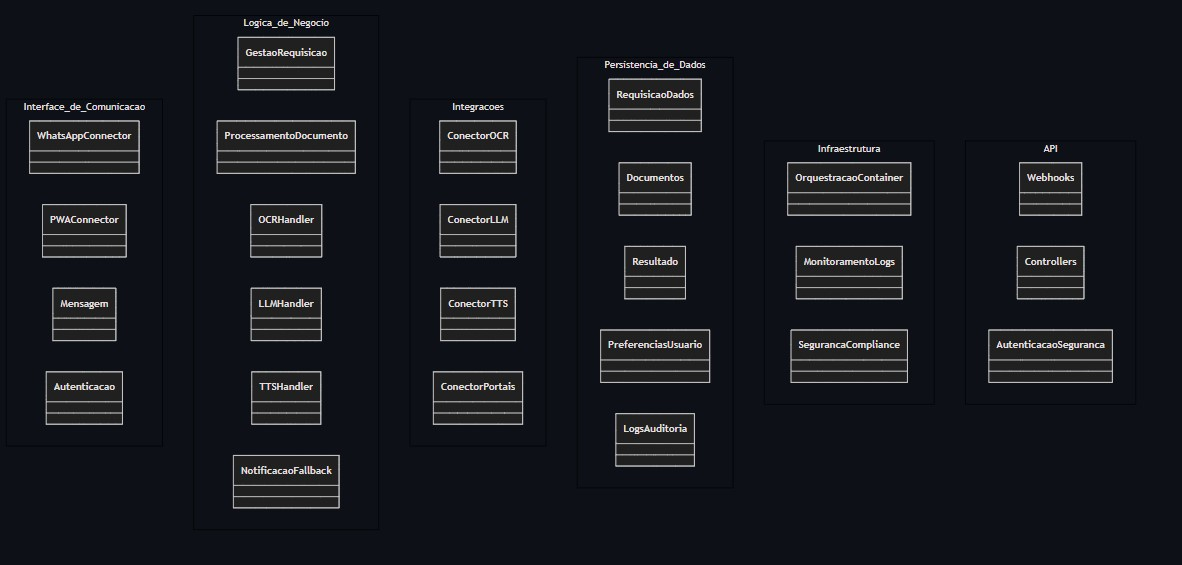
\includegraphics[width=1.4\textwidth,height=7cm,keepaspectratio]{images/Modelo-de-Pacotes.jpg}
\textbf{Observações de DevOps: } Apresenta a organização lógica dos módulos do sistema, agrupando classes e componentes relacionados. Cada pacote representa um domínio funcional (ex.: Interface, Negócio, Persistência, Comunicação).

\newpage

\subsection{API (Esboço)}
\begin{itemize}
    \item POST /webhook/whatsapp — recepção de mensagens/eventos do conector.
    \item POST /v1/requests — criação de requisição (documento/nº processo, metadados de consentimento).
    \item GET /v1/requests/{id} — status e resultado (texto/URI de áudio).
    \item POST /v1/requests/{id}/tts — geração/reattempt de áudio.
    \item GET /v1/users/{id}/history — histórico de consultas.
    \item PUT /v1/users/{id}/preferences — atualização de preferências (texto/áudio). Observações: autenticação mínima (token de canal/telefone), rate-limiting, logs/auditoria.
\end{itemize}

\subsection{Rastreabilidade }
\begin{itemize}
    \item RF01/RF02/RF05 → Casos de uso “Simplificar Documento” + Sequência + Classes Requisicao, Documento, Resultado.
    \item RF03/RF06/RF13 → Atores “Portais/Jurisdições” + Sequência (ramo “nº processo”) + Conector JUR.
    \item RF08/RNF11 → Logs/Observabilidade (componentes LOGS), estados, auditoria.
    \item RNF02/RNF05/RNF10 → Sequência (SLA de tempo), Componentes/Deployment (escalabilidade, disponibilidade).
    \item RNF03 → TTS/Preferências; Wireframes acessíveis.
    \item RNF06/LGPD → Modelo de dados (retenção), API (consentimento), Deployment (segurança).
\end{itemize}

\subsection{Heurísticas e Diretrizes Utilizadas}
\begin{itemize}
    \item Casos de uso como narrativa textual essencial e caixa-preta; diagramas auxiliam na visualização, não substituem o texto.
    \item Modelagem leve e iterativa, evoluindo com requisitos de maior valor/risco primeiro.
    \item Protótipos/Wireframes para reduzir retrabalho e alinhar rapidamente com stakeholders.
    \item DevOps/Deployment desde o início: automação, observabilidade e pequenos incrementos entregáveis.
\end{itemize}

\newpage

\section{Pipeline de CI/CD}

\subsection{Pipeline de Integração Contínua (CI/CD)}

O projeto utiliza um pipeline de integração contínua baseado em \textbf{GitHub Actions}, automatizando o processo de compilação do relatório técnico em formato PDF a partir do código-fonte \LaTeX.

A pipeline é acionada automaticamente sempre que ocorre um \textit{push} ou \textit{pull request} na branch \texttt{main}. O fluxo principal está descrito abaixo:

\begin{enumerate}
  \item \textbf{Checkout do Repositório:} A ação \texttt{actions/checkout@v4} clona o repositório para o ambiente de execução.
  \item \textbf{Compilação do Documento:} Utiliza a ação \texttt{xu-cheng/latex-action@v3} para compilar o arquivo \texttt{main.tex} via \texttt{XeLaTeX}, garantindo suporte a caracteres UTF-8 e pacotes modernos. O parâmetro \texttt{-f} é usado para forçar a compilação mesmo com imagens ausentes.
  \item \textbf{Geração de Artefato PDF:} Após a compilação, o artefato resultante \texttt{main.pdf} é armazenado no GitHub como \texttt{IADvogado-report}, permitindo seu download direto na aba de artefatos do workflow.
\end{enumerate}

Esse pipeline garante reprodutibilidade, rastreabilidade e integração contínua entre a documentação e o código-fonte do sistema. O processo está descrito conceitualmente na Figura~\ref{fig:pipeline-ci}.

\begin{figure}[H]
\centering
\begin{verbatim}
name: Build LaTeX Document
on:
  push:
    branches: [ "main" ]
  pull_request:
    branches: [ "main" ]
jobs:
  build_pdf:
    runs-on: ubuntu-latest
    steps:
      - uses: actions/checkout@v4
      - uses: xu-cheng/latex-action@v3
        with:
          root_file: main.tex
          latexmk_use_xelatex: true
          args: -f
      - uses: actions/upload-artifact@v4
        with:
          name: IADvogado-report
          path: main.pdf
\end{verbatim}
\caption{Pipeline de integração contínua para compilação automática do relatório.}
\end{figure}


\newpage

\subsection{Próximos Passos de Modelagem}
\begin{enumerate}
    \item Detalhar texto completo dos Casos de Uso prioritários (incluindo pré/pós-condições, regras de negócio e exceções).
    \item Refinar sequência com tempos de resposta máximos e fallback claros.
    \item Versão 2 do ER (normalização, índices de busca por nº de processo, partição de histórico).
    \item Protótipo navegável (baixa/alta fidelidade) para testes moderados com usuários.
    \item Métricas de qualidade acopladas ao modelo (SLA, taxa de falha, cobertura de logs).
\end{enumerate}

\section{Repositório}
Todo o conteúdo detalhado deste projeto, incluindo documentação, código e materiais adicionais, encontra-se disponível no repositório oficial no GitHub: \href{https://github.com/BrunoAG77/IADvogado}{github.com/BrunoAG77/IADvogado}.

\end{document}
